\chapter{ILD Global Integration}
\writer{Karsten Buesser, Claude Vallee}

\vspace{2cm}

\section{Internal ILD integration}
\writer{Karsten Buesser, Roman Poeschl, Toshiaki Tauchi}{3}

Subdetector interfaces and integration scheme including services. Short reminder of the overall ILD integration scheme (unchanged). Technical drawings (ideally from CAD files) showing interfaces (pipes, cables, supports) for each subdetector within ILD. New input is expected from the recently setup dedicated working group chaired by Roman to update the service paths based on subdetector Interface and Control Documents.

Among points to illustrate: Inner tracker services, TPC services, ECAL electrical interfaces, HCAL interfaces in TESLA option and Videau option, VFS cables, global scheme for cable paths.   

\vspace{2cm}

\section{External ILD integration}
\writer{Yasuhiro Sugimoto}{1}

Generic layout of the cavern, mentioning the current options for its configuration (TDR, Tohoku, YS).

\vspace{2cm}

\subsection{Cavern ancillary services}
\writer{Yasuhiro Sugimoto}{1}

Summary of ancillary services from subdetectors in the cavern and on surface, as it will result from subdetector information to be provided in 
Yasuhiro's excel file.

ILD overall wish for utility space
on the platform, the service gallery 
and the service cavern.

\vspace{2cm}

\subsection{Data acquisition}
\writer{Matthew Wing, Taikan Suehara}{2}

Expected principles and sketch of the DAQ.

Summary of characteristics of subdetector data including data throughput and local filtering, 
based on DAQ information recently requested to all subdetectors.

EUDAQ developments towards combined DAQ systems for beamtests

\vspace{2cm}

\section{Mechanical structure and studies}
\writer{Felix Sefkow, Henri Videau, Karsten Buesser, Roman Poeschl, Toshiaki Tauchi}{3}
\label{ild:sec:mechanical_structures}

Static deformations of both structure options (TESLA/Videau) including LLR-DESY crosscheck.

Dynamic behaviour of both structure options under reference earthquake spectra, including LLR-DESY crosscheck.

New insights on the above issues are expected from the dedicated group steered by Henri, Felix, Roman and Karsten. Crosschecks between DESY and LLR will most likely restrict to the barrel. A discussion of the endcap structure may also be included. 

If available, results on the mechanical behaviour of other subdetectors (e.g. TPC) are also welcome.

\vspace{2cm}

\section{Coil and yoke studies}
\writer{Karsten Buesser, Uwe Schneekloth}{3}

Baseline yoke design and discussion of possible lighter options including separation wall option.

Updated field maps for the baseline yoke design. Table of field maps at various locations (including stray fields) for various yoke options.

Progress on technological design of anti-DID (KEK/Toshiba/Hitachi) and corresponding field map.

\vspace{2cm}

\section{Beam background studies}
\writer{Daniel Jeans, Yan Benhammou, Sergej Schuwalow}{2}

Beam-beam BG occupancies with/without anti-DID. New results are expected from Daniel soon to clarify the open points of previous studies and consolidate the estimations. The rates shown in the IDR should if possible be computed for the latest ILC250 beam conditions (input files available from Anne Schuetz).

It would also be good to provide hit maps from backscattered neutrons from the beamdump and from halo muons, possibly using input particle files from Anne Schuetz.

\vspace{2cm}

\section{Alignment/ calibration procedures}
\writer{Graham Wilson}{1}

There was little progress here since the LOI/DBD. Most of the corresponding text of these documents could be recovered and summarized for the IDR, taking into account the latest considerations about in-situ calibration with particles/collisions and subdetector requirements.

\vspace{2cm}

\section{Technical Documentation}

The technical description of the ILD detector concept comprises specification and design documents as well as 3d engineering models, interface descriptions and drawings. All these documents that form the backbone of the ILD technical documentation are stored in the ILC Engineering Data Management System ILC-EDMS~\cite{ild:bib:edms}. As this powerful system is made for experts and requires appropriate attention, an easy accessible frontend ("EDMSdirect") has been made available. The ILD technical documentation is organised in a Work Breakdown Structure (WBS) that is mapped on a tree browser that can be accessed on the web~\cite{ild:bib:edmsdirect}. Figure~\ref{ild:fig:integration:edmsdirect} shows the tree browser for the ILD technical documentation. All WBS top nodes can be expanded by clicking on them. In the figure, this has been done for the node "Design Integration".


\begin{figure}[t!]

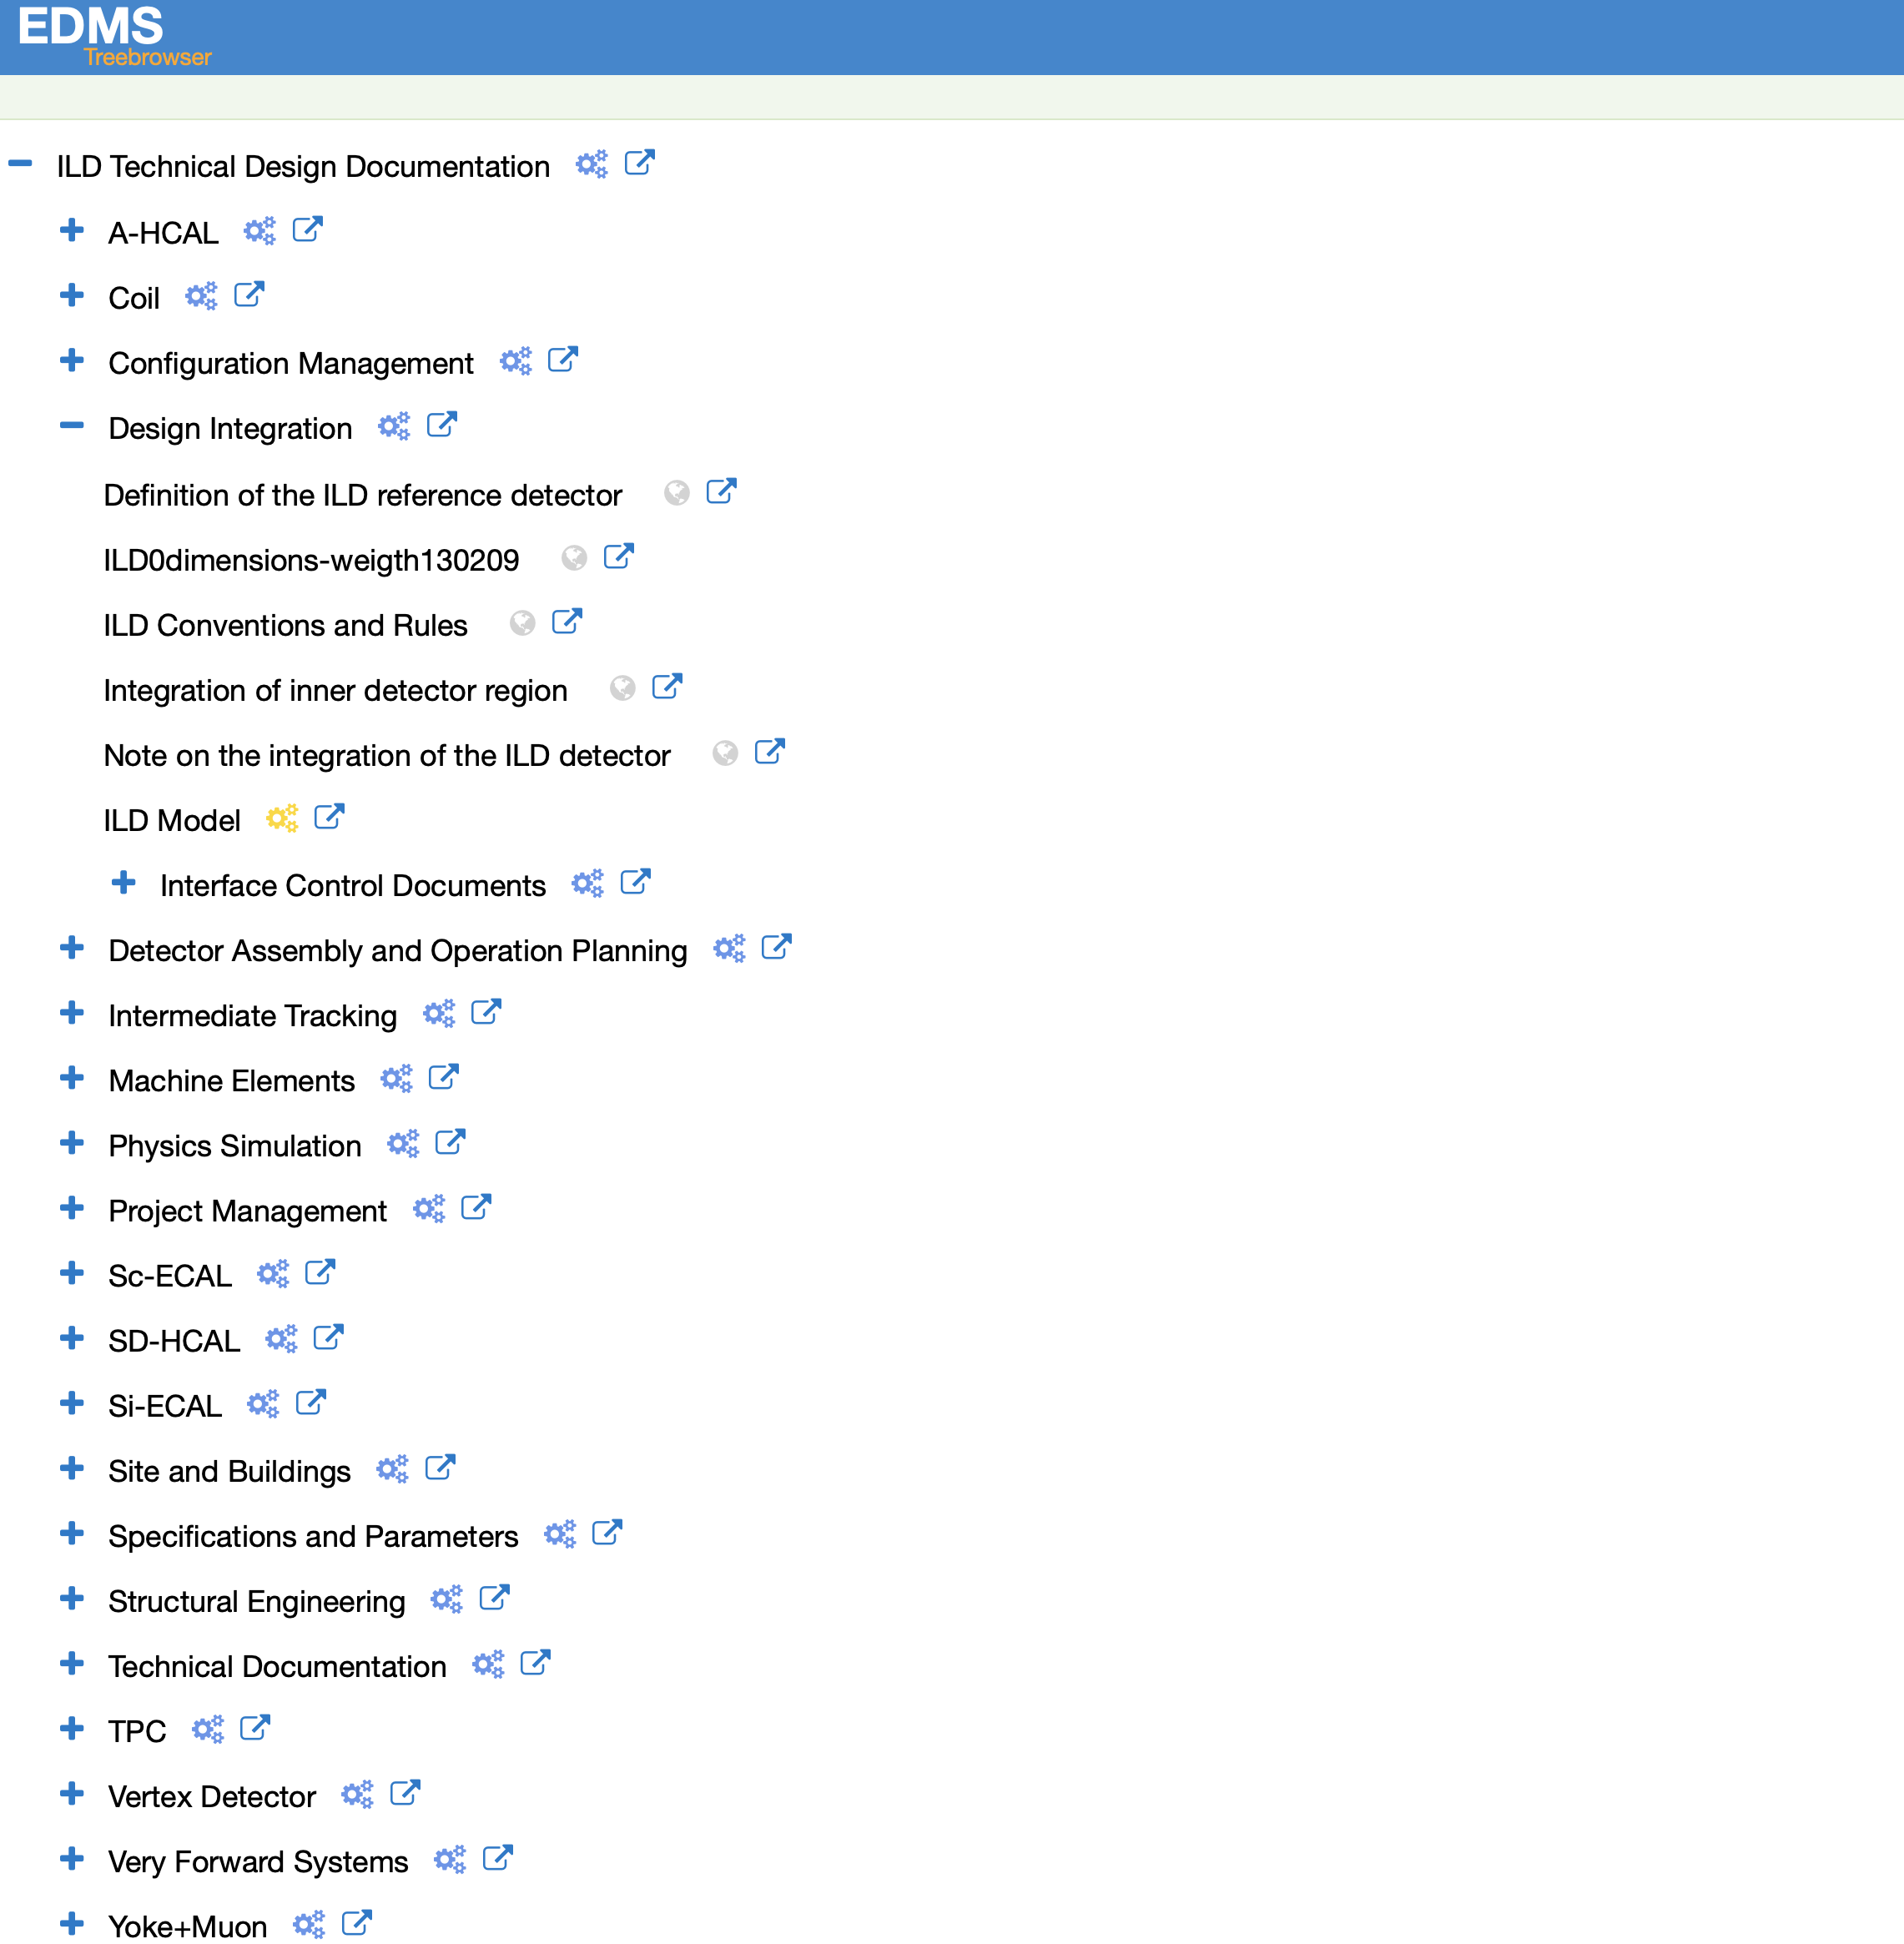
\includegraphics[width=0.8\hsize]{Integration/fig/EDMS_direct.png}

\caption{\label{ild:fig:integration:edmsdirect}Treebrowser of the ILD technical documentation Work Breakdown Structure in the ILC Engineering Data Management System. The top level node "Design Integration" is shown expanded.}
\end{figure}

Figure~\ref{ild:fig:integration:edmsdirect_document} shows the document browser that opens for the documents stored in the EDMSdirect system. Shown here is the "Conventions and Rules" document that belongs to the previous mentioned WBS node "Design Integration". A preview of the document is shown in the document browser. The document browser allows for preview of the respective documents as well as downloads of pdf or source files, depending on the authorisation of the users. Documents can be made worldwide visible as well as protected for selected users.

\begin{figure}[t!]

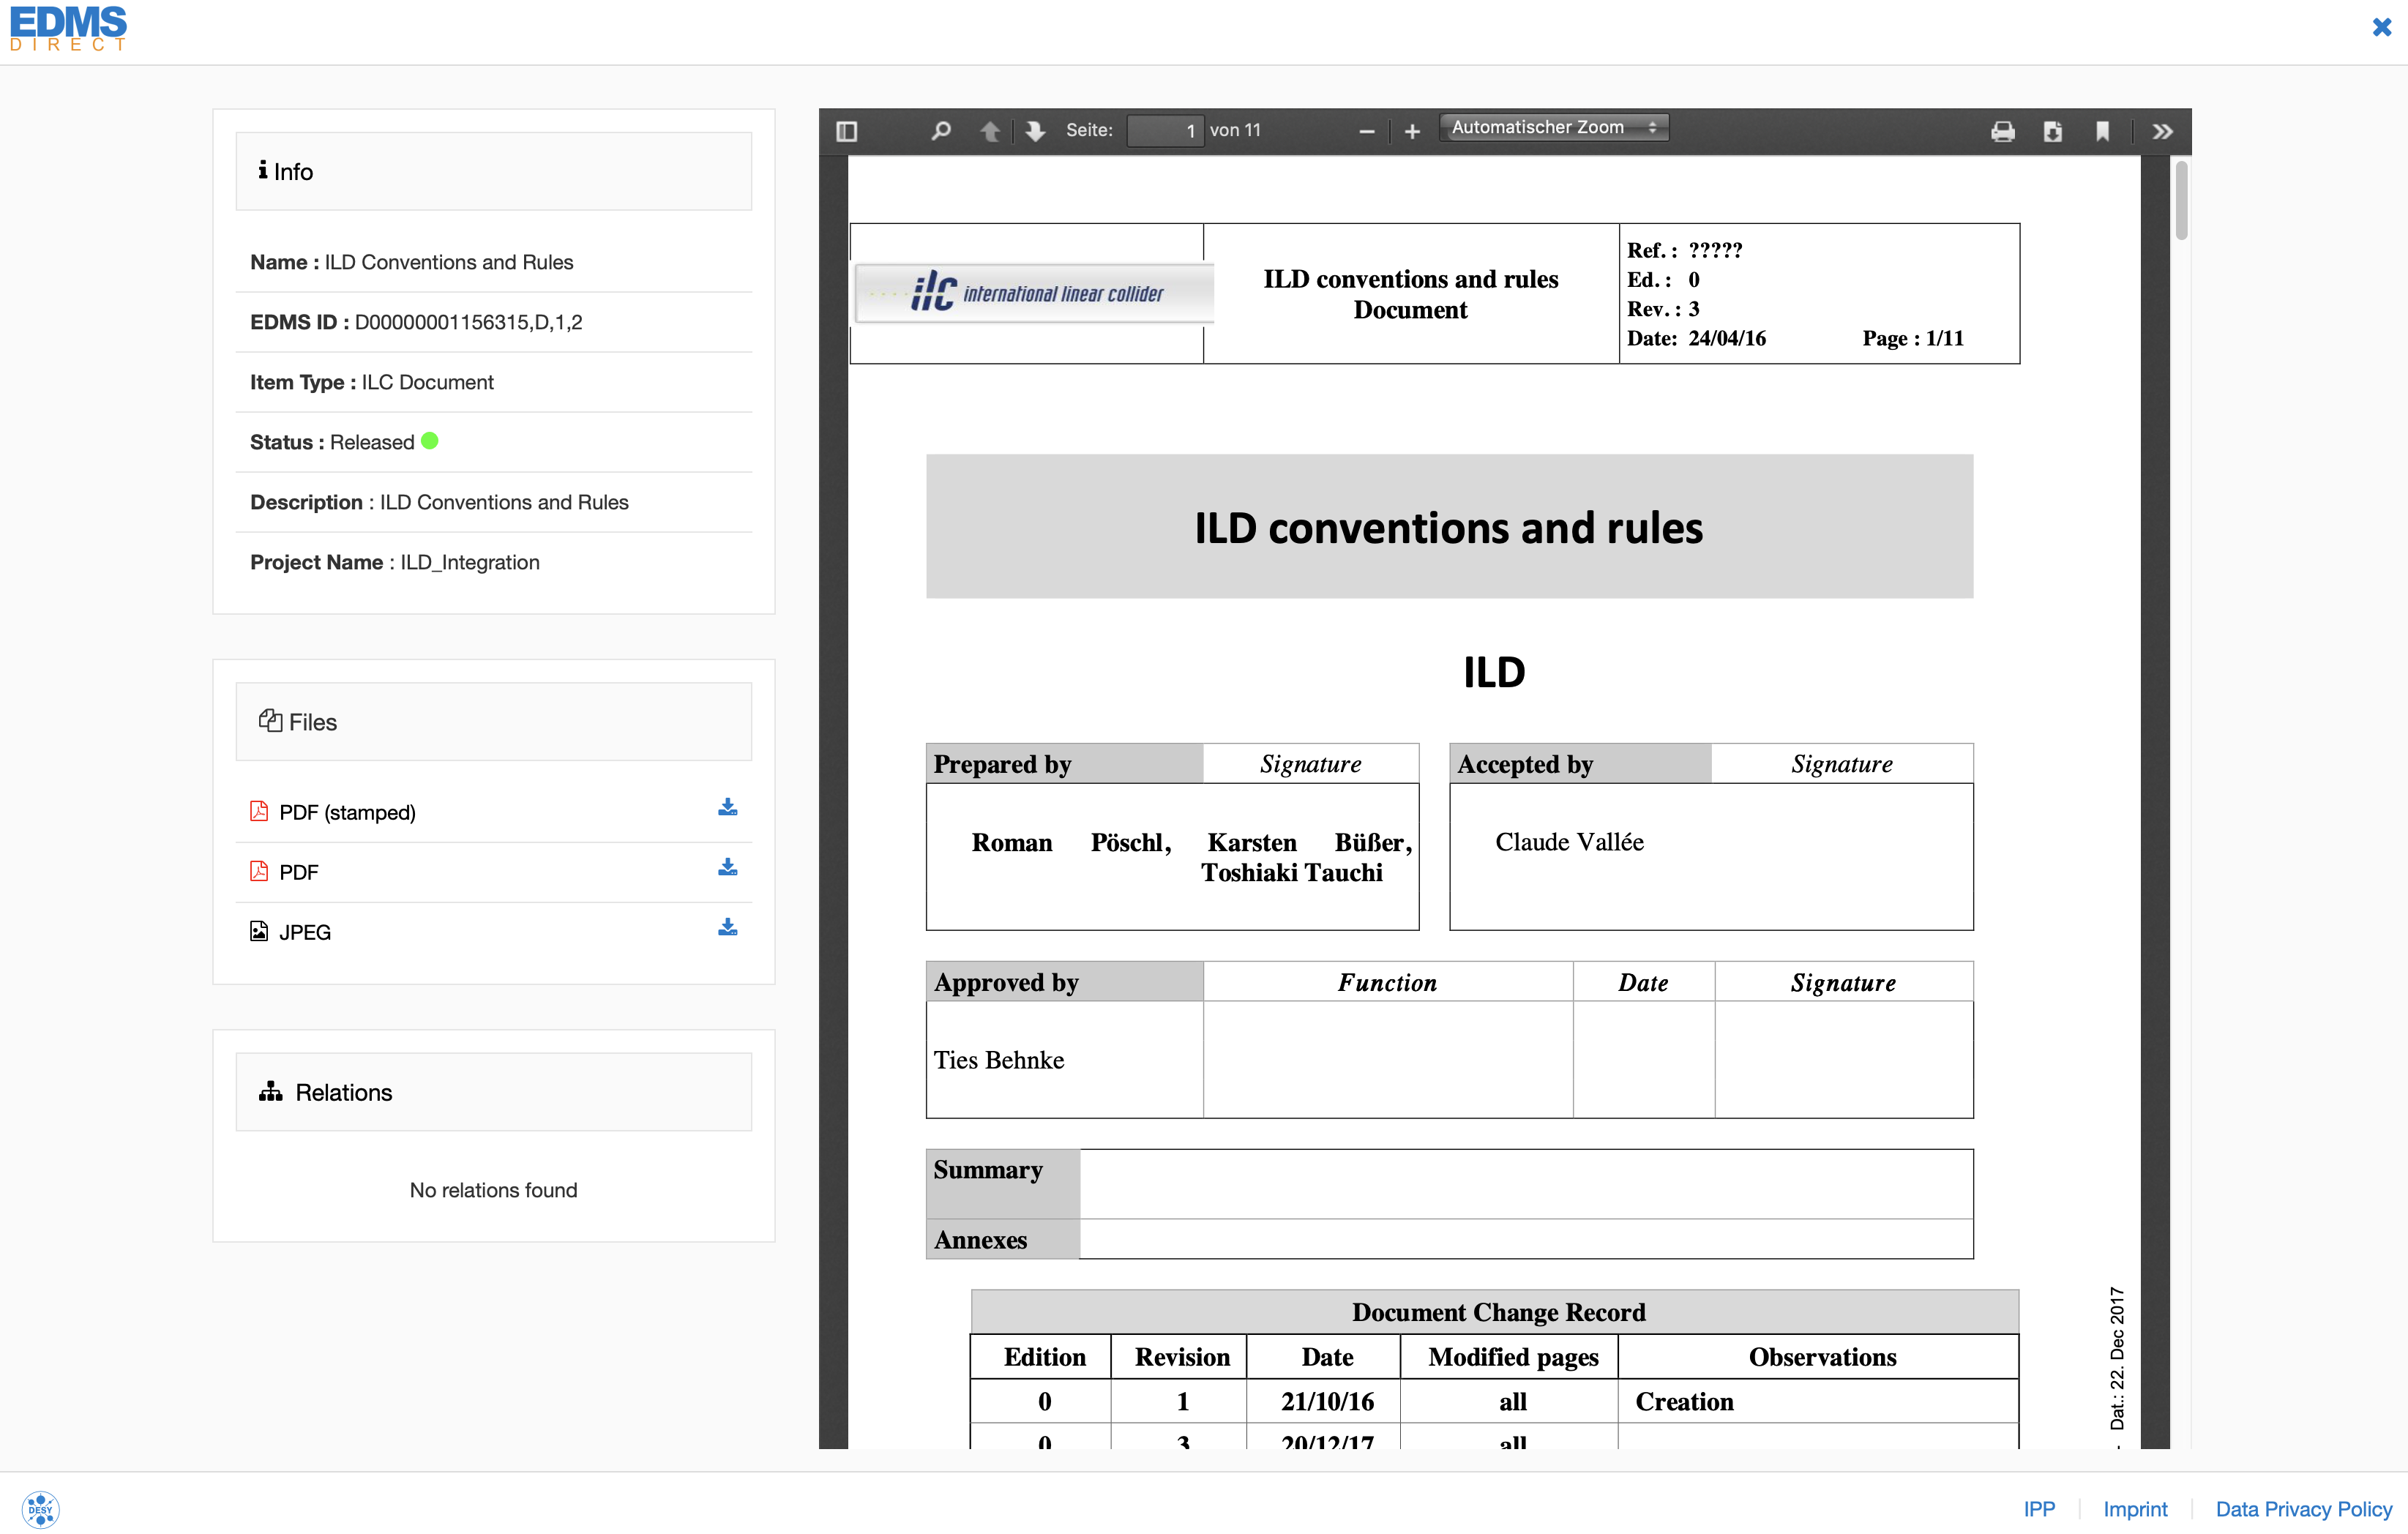
\includegraphics[width=0.8\hsize]{Integration/fig/EDMS_direct_document.png}

\caption{\label{ild:fig:integration:edmsdirect_document}Example document (here:"ILD Conventions and Rules") in the document browser of EDMSdirect.}
\end{figure}

\subsection{Interface Control Documents}


\section{Earthquake Safety}
Japan is one of most seismically active regions in the world. The proposed sit for the ILC in the Kitakami mountains of northern Honshu has been especially selected putting emphasis on benign seismic conditions. Earthquake history has been taken into account as well as recent surveys on active tectonic faults. Nevertheless, earthquakes can occur and need to be taken into account. Figure~\ref{ild:fig:integration:earthquake_map} shows all earthquakes that were detected during 30 days in winter 2019/2019 in northern Honshu. The ILD interaction region is in a relatively quiet region around (39N, 141,5E).

\begin{figure}[ht]
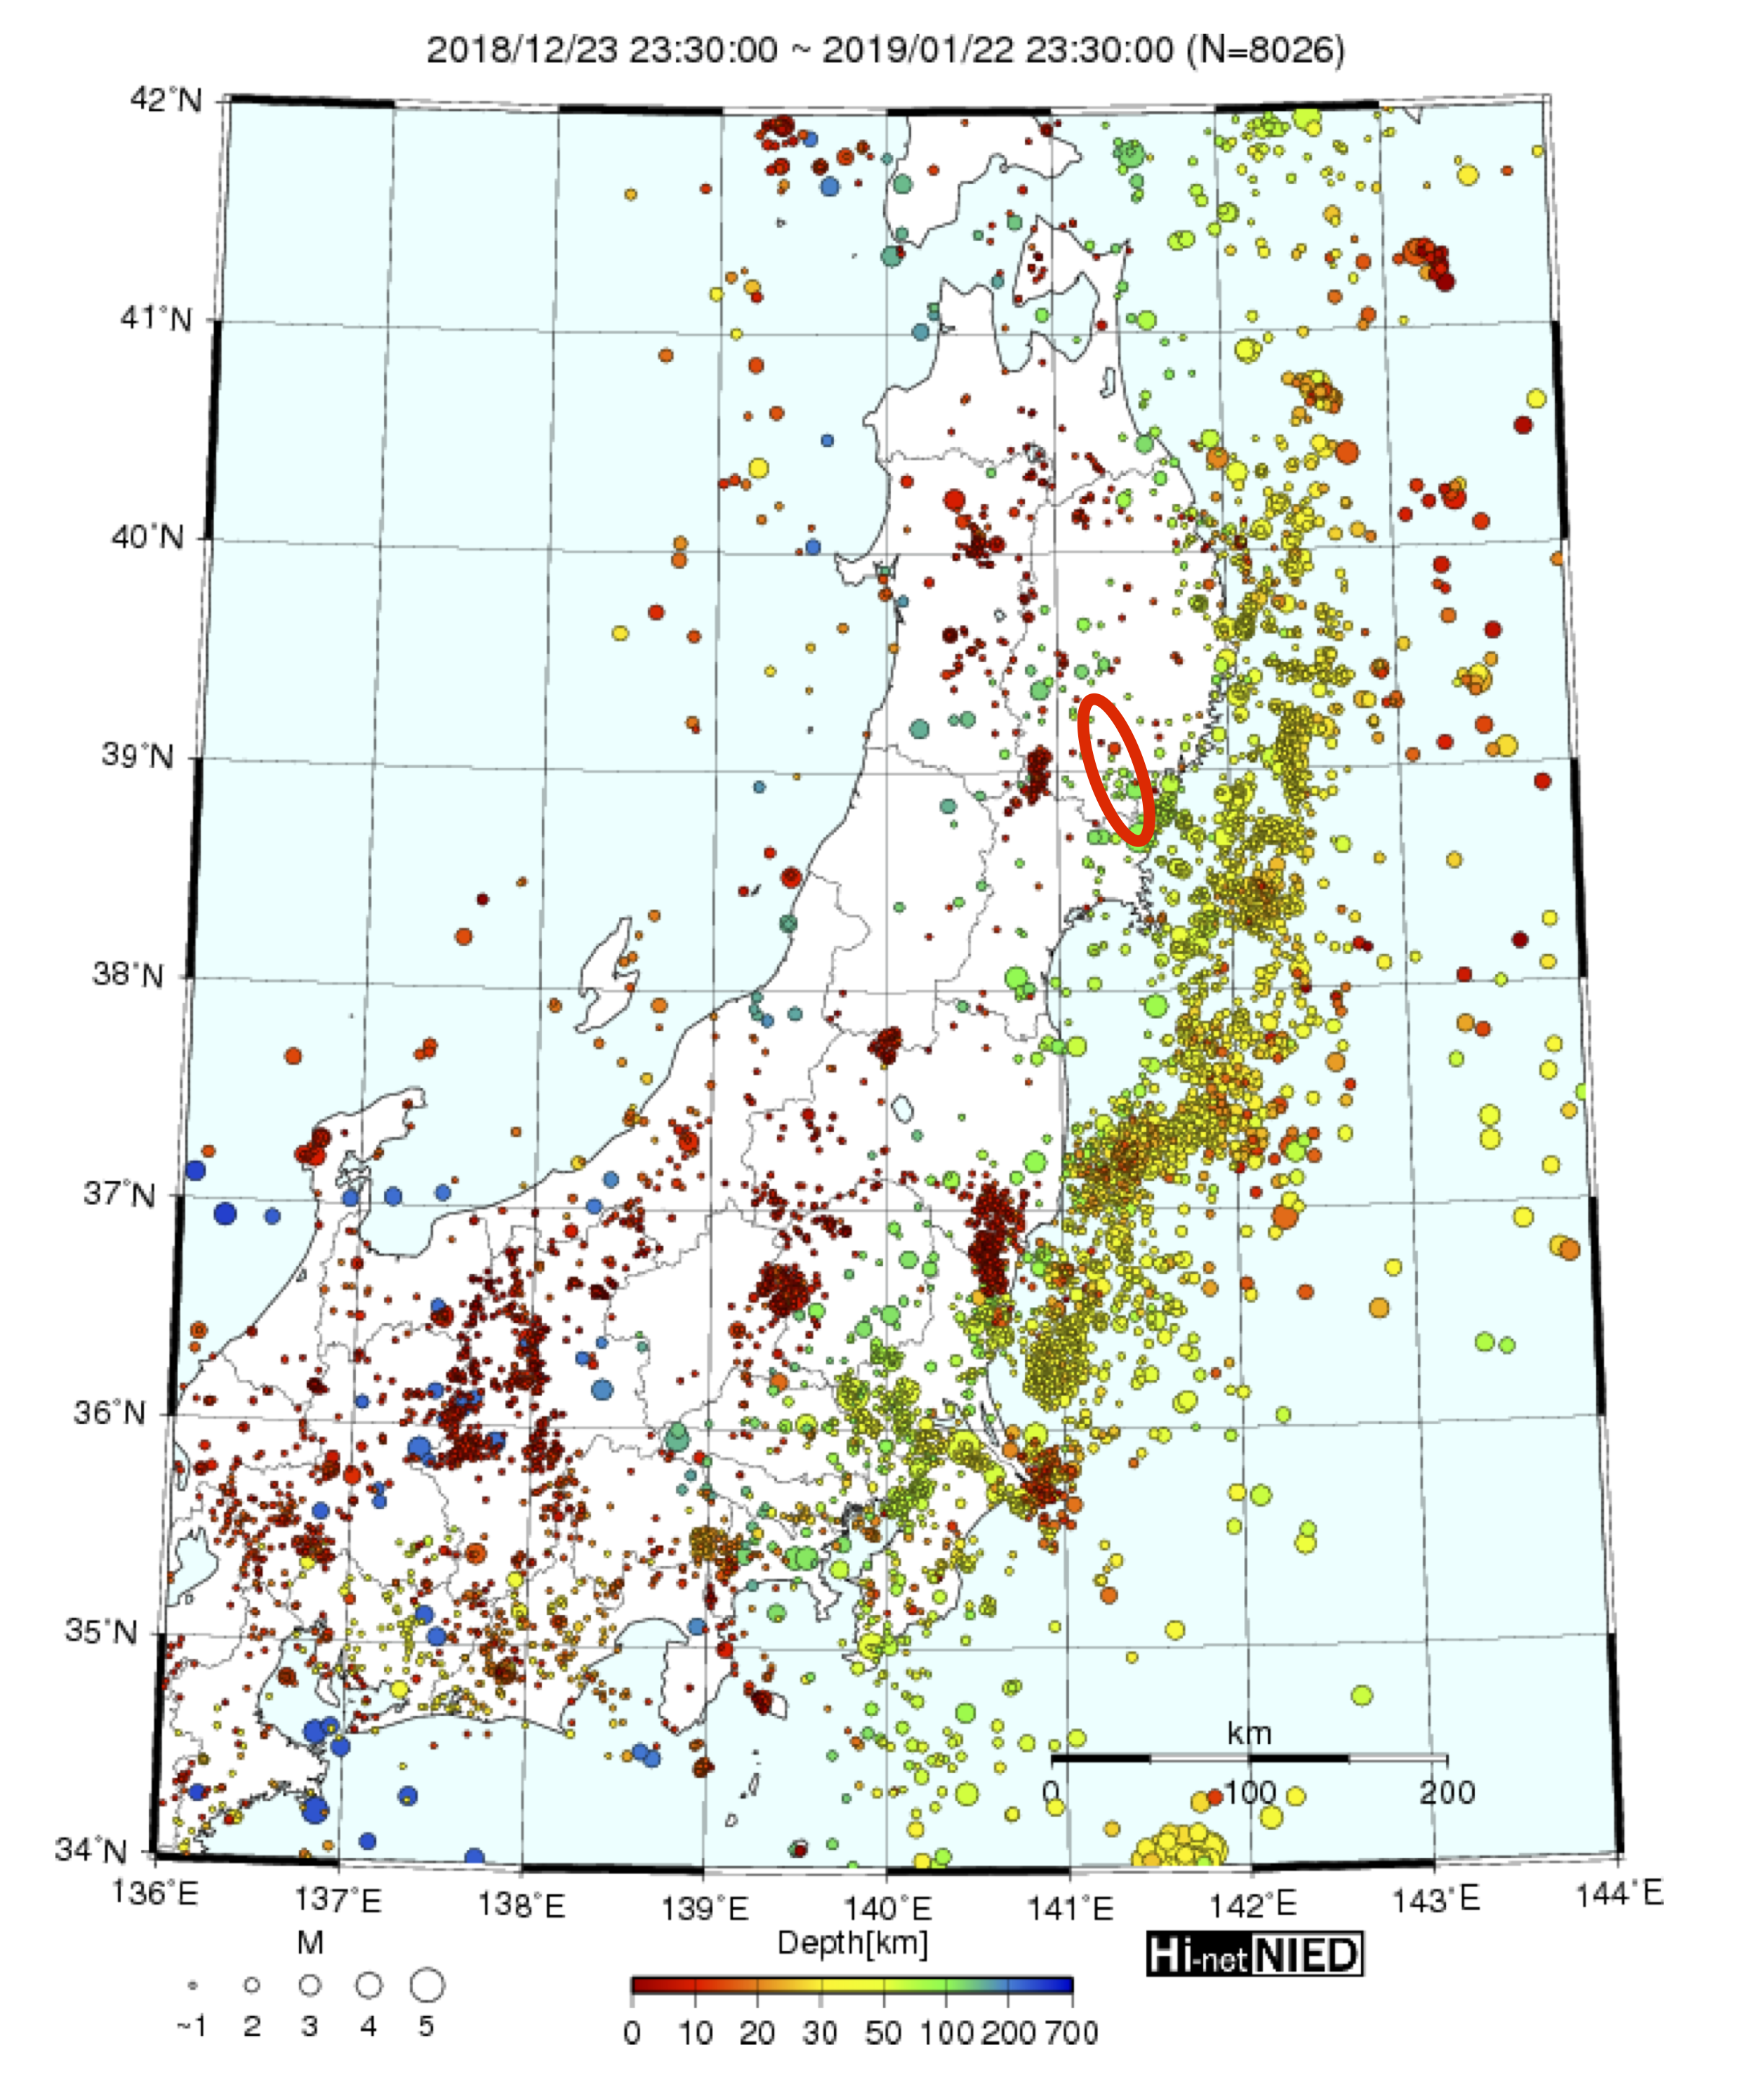
\includegraphics[width=0.8\hsize]{Integration/fig/earthquake_map.png}

\caption{\label{ild:fig:integration:earthquake_map}Map of northern Honshu with all detected earthquakes between 23rd December 2018 and 23rd January 2019 (30 days)~\cite{ild:bib:hi-net}. The ILC interaction region is close to coordinates (39N, 141.5E)}
\end{figure}

\subsection{Structural Design}

Emphasis has been put on the design of the ILD detector with respect to earthquake safety in view of operability of the detector as well as disaster prevention. General rules are provided by the ISO3010 standard: "Bases for design of structures -- seismic actions on structures". The ISO standard states two basic principles:
\begin{itemize}
\item The structure should not collapse nor experience other similar forms of structural failure due to severe earthquake ground motions that could occur at the site (ultimate limit state: ULS).
\item The structure should withstand moderate earthquake ground motions which may be expected to occur at the site during the service life of the structure with damage within accepted limits(serviceability limit state: SLS).
\end{itemize}
As guidance rules, ULS events are those which are expected to happen with recurrence rates of 500~years, while SLS events might happen every 20~years. For the envisaged ILC site in Kitakami this corresponds to maximum expected accelerations of $\approx$150~gal and $\approx$450~gal. 

Proper analysis of the ILD mechanical structures is under way using response spectra for standard earthquakes in Kitakami (c.f.~figure~\ref{ild:fig:integration:earthquake_spectra}). Section~\ref{ild:sec:mechanical_structures} gives an overview of the ongoing structural studies for ILD.

\begin{figure}[t!]

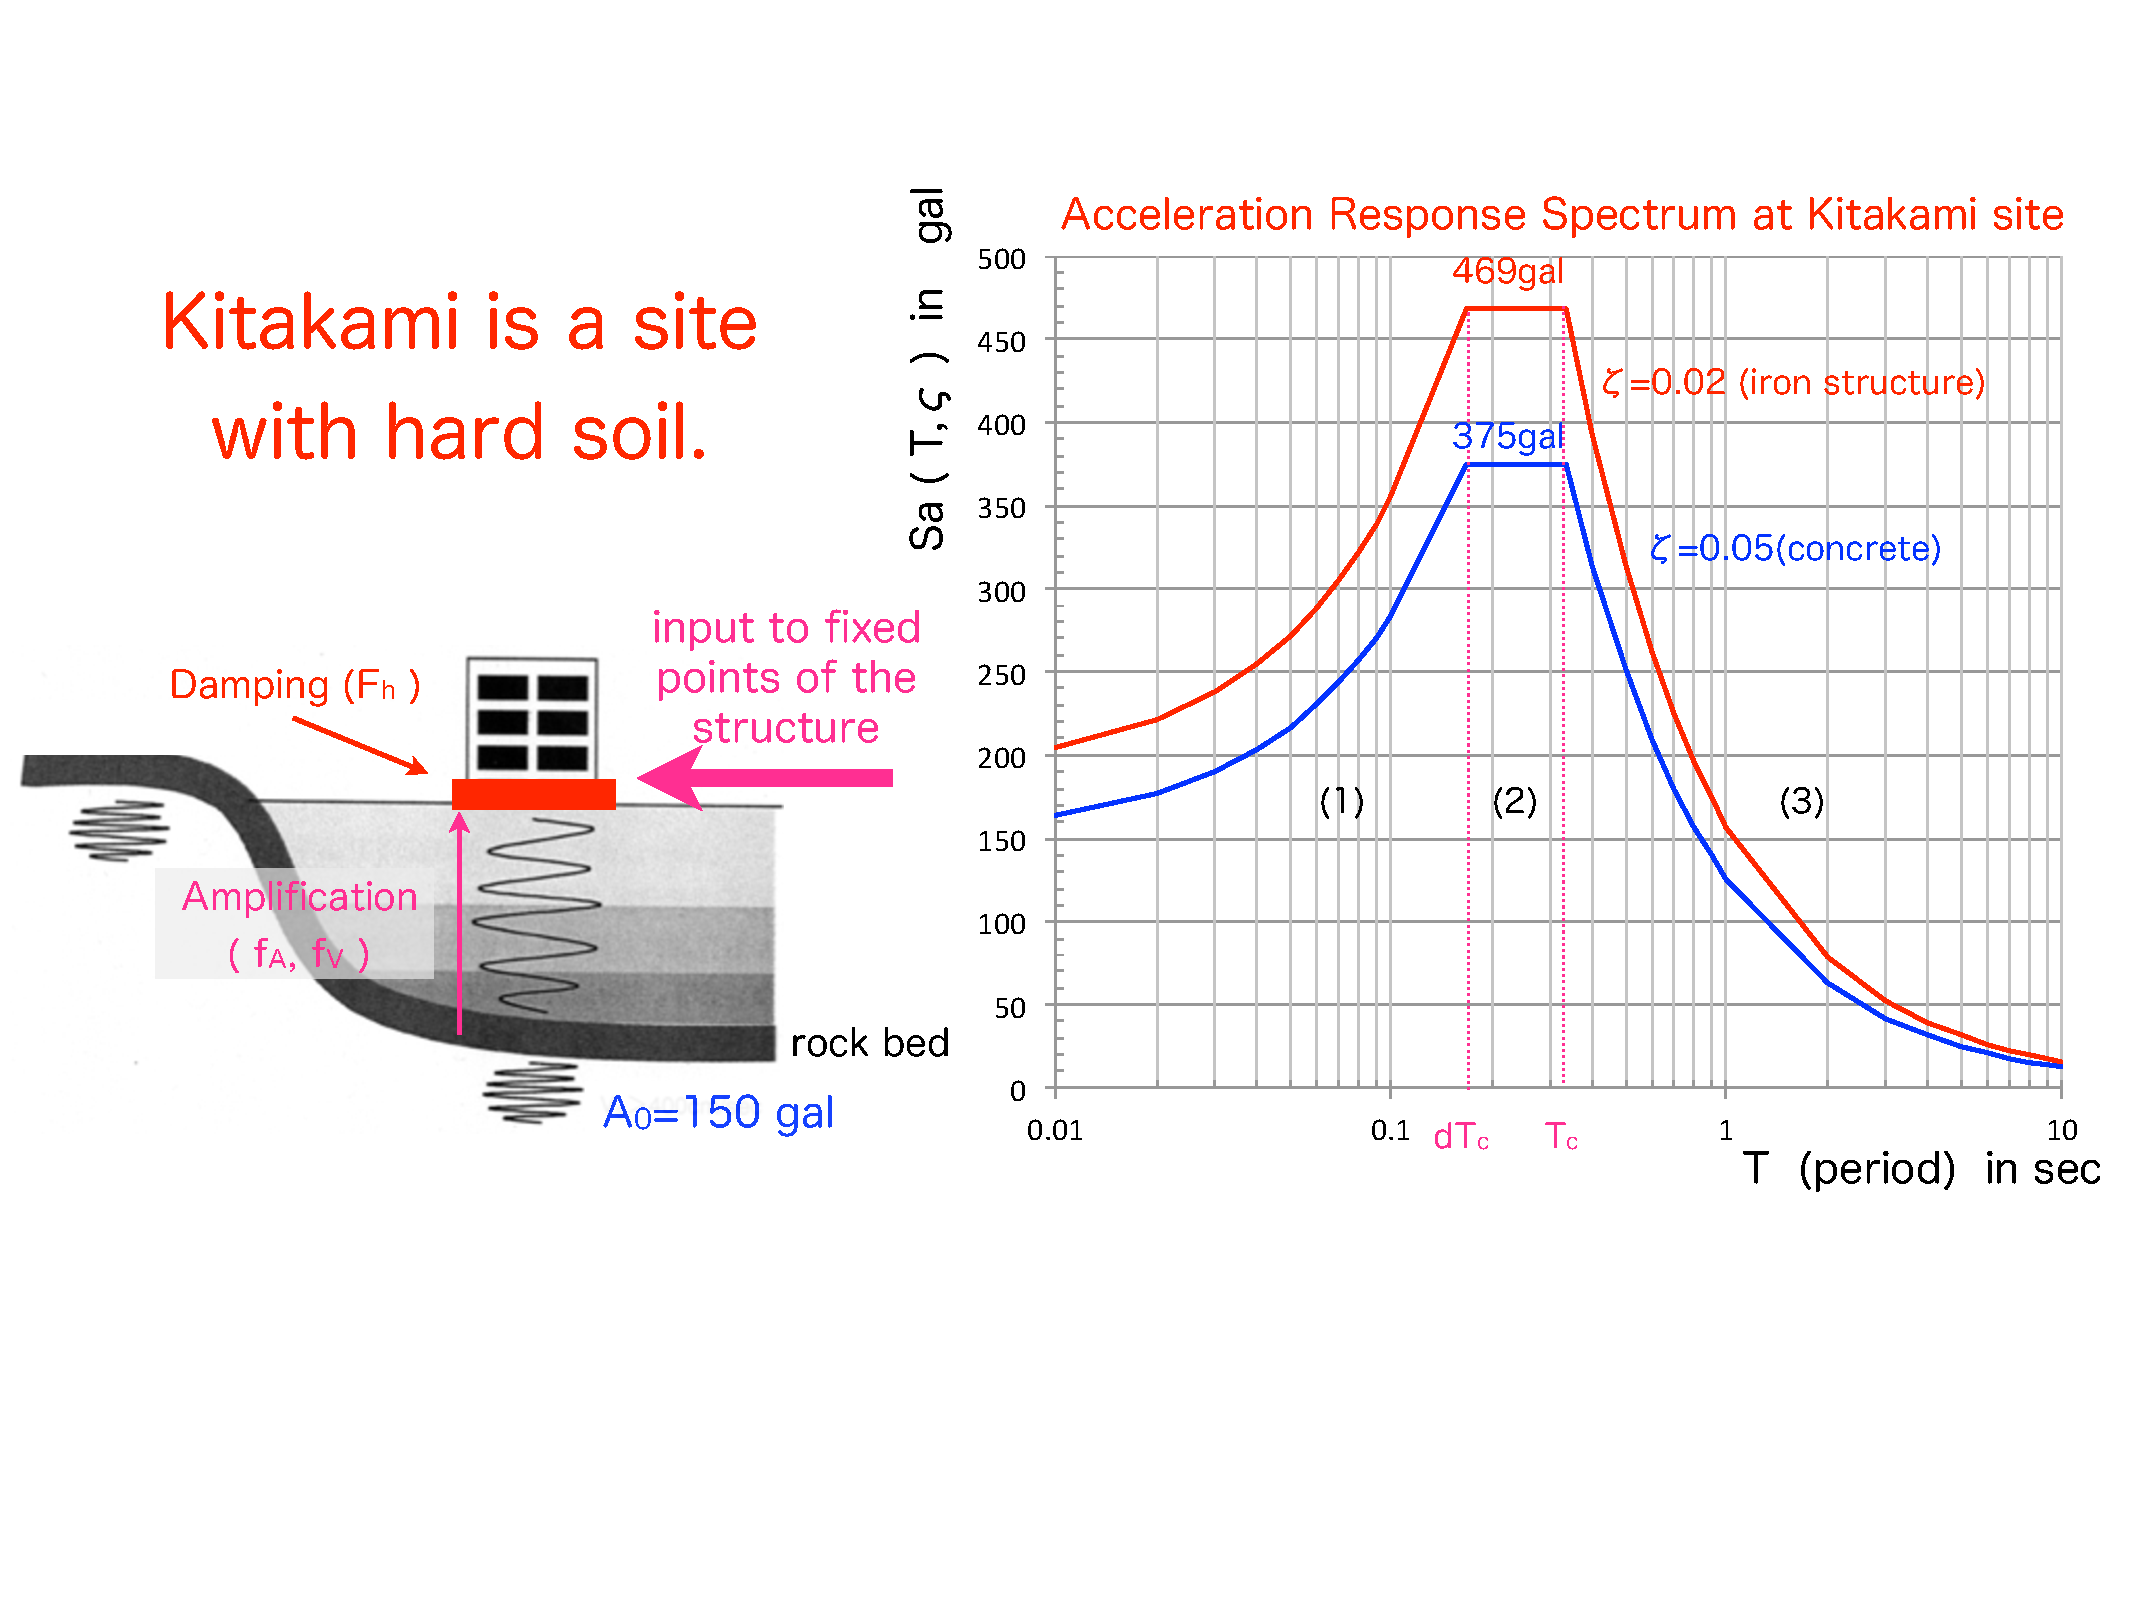
\includegraphics[width=0.8\hsize]{Integration/fig/earthquake_spectra.pdf}

\caption{\label{ild:fig:integration:earthquake_spectra}Standard response spectra for earthquakes in Kitakami (hard soil) for structures with different damping behaviour~\cite{ild:bib:earthquake}. A maximum acceleration of 150~gal for an earthquake with a recurrence frequency of 100~years has been assumed.}
\end{figure}

\subsection{Seismic Isolation}


